% !TeX root = Tesis.tex

\chapter{Marco Teórico}
\section{La teoría de la carga cognitiva y las emociones}

La tecnología ha permitido que se introduzcan nuevas formas de estudio en los diversos campos, por ejemplo, en la psicología cognitiva recientemente se han realizado diversas investigaciones para la detección de la carga cognitiva.  La carga cognitiva es el esfuerzo de la memoria de trabajo al realizar una tarea específica. La memoria de trabajo representa la capacidad de aprender, sin embargo, tiene sus limitaciones. 

La Teoría de la Carga Cognitiva (TCC), se basa en reconocer que la memoria de trabajo tiene un capacidad limitada de almacenamiento de la información, la memoria de trabajo se refiere al esfuerzo necesario del cerebro para procesar información al realizar una tarea específica. Por lo tanto el proceso de aprendizaje se lleva a cabo de manera exitosa si se evita la sobrecarga de la memoria a corto plazo \cite{sweller}.

Existen tres tipos de carga cognitiva: la intrínseca, la extrínseca y la germánica. La carga cognitiva intrínseca está relacionada con la complejidad de la tarea a realizar y los conocimientos previos con los que se cuenta. La carga extrínseca o extraña se refiere a proporcionar información innecesaria lo que puede dificultar la realización de la tarea. Finalmente la carga cognitiva germánica o pertinente es emplear eficientemente los recursos de la memoria de trabajo lo que aumenta el proceso de abstracción \cite{cardenas}. 



Por otra parte, las emociones tienen ciertas implicaciones en el aprendizaje; las emociones ayudan a fomentar el aprendizaje, ya que pueden estimular la actividad de las redes neuronales, en consecuencia los conocimientos se adquieren de una manera más fácil.  La emoción es un proceso psicológico que se da en los seres humanos para que puedan adaptarse y responder al entorno.   
La emoción sed define como el proceso que ``implica una serie de condiciones desencadenantes (estímulos relevantes), diversos niveles de procesamiento cognitivo (procesos valorativos), cambios fisiológicos (activación), patrones expresivos y de comunicación (expresión emocional)'' \cite{garcia}.

\section{Señales bioeléctricas}

Una señal es  un medio de transmisión de información, su adquisición permite obtener información relevante sobre los que se desea estudiar. En el caso de bioseñales se refiere a las señales generadas por los diferentes sistemas fisiológicos del organismo. Gómez-Díaz, Villalobos-Torres, Lara-Rendón, Juarez-Guerra, Castellanos-Nolasco, Ortiz-Gaucín, Suarez-Gómez (2018).

Las señales bioeléctricas  representan variables fisiológicas que son relevantes para la generación de interfaces más naturales entre un ser humano y una máquina. A partir de tales señales se pueden evaluar patrones de comportamiento durante la interacción humano-computadora.\cite{ray} Existe una gran variedad de señales bioeléctricas, a continuación se describirán cada una de ellas.


\begin{figure}[htb]
	\centering
	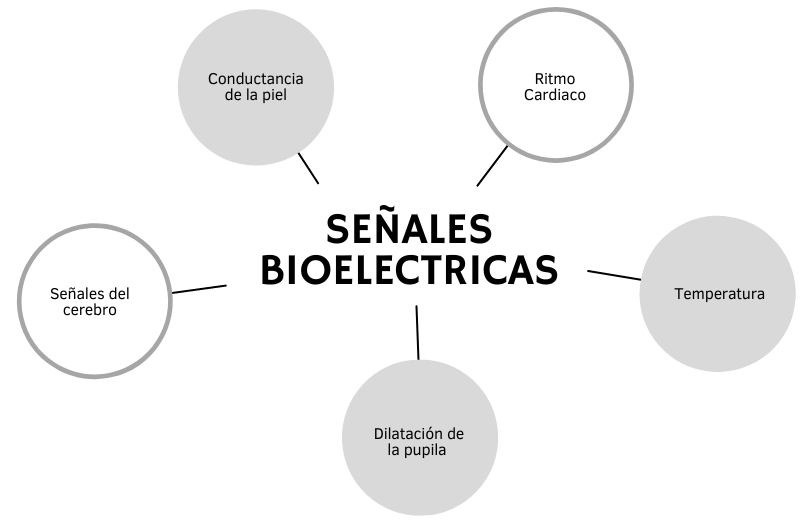
\includegraphics[width=\textwidth]{imagenes//bioseñales.png}
	\caption{Señales bioelectricas}\label{f:fig1y2}
	Fuente: Elaboración propia
\end{figure}

\subsection{Señales del cerebro}
Las neuronas cerebrales se comunican a través de señales eléctricas que se pueden medir. A esto se le conoce como ondas cerebrales. Estas ondas son detectadas mediante un estudio de electroencefalograma  (EEG), el cual detecta cambios en la actividad cerebral que pueden ser útiles para diagnosticar trastornos cerebrales.  

\subsection{Señales de conductancia de la piel}

La actividad electrodérmica se define como el cambio en las propiedades eléctricas de la piel. También conocida como respuesta galvánica de la piel (GSR, Galvanic Skin Response por sus siglas en inglés). En este método, la conductancia eléctrica de la piel se mide a través de uno o dos sensores o electródos usualmente unidos a una parte de la mano o el pie.

	

\subsection{Señales de Ritmo Cardiaco}
Según la OMS, las señales de ritmo cardíaco o frecuencia cardíaca son las pulsaciones del corazón por minuto. 
La frecuencia cardiaca (FC) en reposo oscila entre 50 y 100 latidos por minuto en las personas adultas. Al nacer, la FC es más elevada porque el bebé la necesita para su adecuado crecimiento. A partir del primer mes de vida, la FC va disminuyendo hasta alcanzar las cifras normales de un adulto. 
	El ejercicio físico o las situaciones de estrés provocan un aumento de la FC (taquicardia sinusal), que se considera normal. La FC máxima que un corazón normal puede alcanzar durante un ejercicio físico intenso se puede calcular con la siguiente fórmula: FC máxima = 220 – edad.

El electrocardiograma (EKG o ECG) es un tipo de señal bioeléctrica producidas en el corazón, la obtención de ella evalúa el ritmo y la función cardiaca a través de un registro de la actividad eléctrica del corazón, es muy útil para determinar si una persona sufre de enfermedad cardiaca y si el corazón está latiendo normalmente \cite{wilches}

\subsection{Señales de Temperatura}
La temperatura corporal es la medida obtenida a partir de la capacidad del organismo de generar y eliminar calor. \cite{wilches}. 


\subsection{Señales de Dilatación de la pupila}

La pupila es el orificio negro que hay en el ojo, en el centro del iris, que tiene la capacidad de contraerse y dilitarse para controlar la entrada de luz a la retina. La dilatación pupilar es una de las señales fisiológicas generadas por el organismo. La dilatación de la pupila también es el reflejo del estado emocional en una persona, ya sea positivo o negativo. (Aracena Cornejo, 2014).

\section{Sensado de señales}

El término “sensor” se emplea para los dispositivos que convierten una medida física en una señal eléctrica. En el mercado existen un gran variedad de sensores empleados para la medición de señales que genera el cuerpo humano.

Algunos de estos se mencionan a continuación: 

\subsection{Sensores Shimmer}
Los sensores portátiles de Shimmer permiten capturar datos cinemáticos y biofísicos de manera simple y efectiva en tiempo real en diversas áreas de aplicación. 

\begin{figure}[htb]
	\centering
	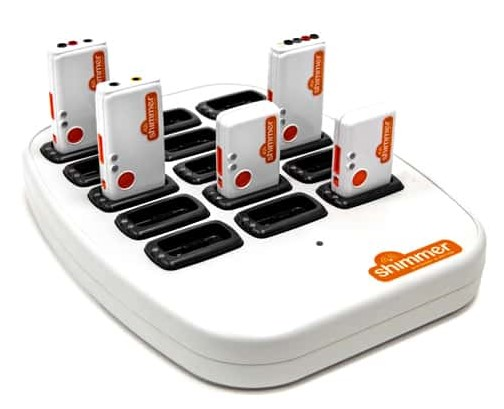
\includegraphics[width=\textwidth]{imagenes//sensores_shimmer.jpg}
	\caption{Sensores Shimmer3}
\end{figure}

\subsubsection*{ Sensores Shimmer IMU} 

Sensor inalámbrico potente proporciona datos de calidad a través de sensores de aceleración, giroscopio, mag y presión. Este tipo de sensores fue utilizado por Investigadores de la Universidad de Gotemburgo, para dar seguimiento a personas con epilepsia y  enfermedad de Parkinson. 
\subsection*{ Sensores Shimmer electrocardiograma} 

Los sensores de electrocardiograma (ECG) Shimmer 3 Consensys se pueden utilizar para monitorear cuatro canales de ECG. Este tipo de dispositivos portátiles se han utilizado para el registro de varios componentes de la actividad diaria. Principalmente para monitorear  la actividad física en las personas mayores y detectar posibles enfermedades.

\subsection*{Sensores Shimmer GSR, ECG y EEG} 

Estos sensores han sido de utilidad para determinar rasgos de personalidad que son parámetros fundamentales para caracterizar el comportamiento de un individuo.  Los rasgos de personalidad se analizan estadísticamente y se reconocen mediante señales fisiológicas GSR, ECG y EEG. Se han realizado estudios de IHC para determinar patrones de satisfacción del cliente con el producto final.

\subsection{BITalino} 

BITalino es un kit electrónico que integra varios módulos individuales, que sirve para la obtención de señales fisiológicas. Este kit contiene un microprocesador que se encarga de convertir las señales analógicas a señales digitales. BITalino cuenta con sensores diseñados específicamente para obtención de señales EDA, ECG, EEG y EMG. Además agrega un acelerómetro y  un sensor de luminosidad.

BITalino cuenta con su propia plataforma de software denominada OpenSignals para monitoreo y obtención de los datos biométricos. 
\begin{figure}[htb]
	\centering
	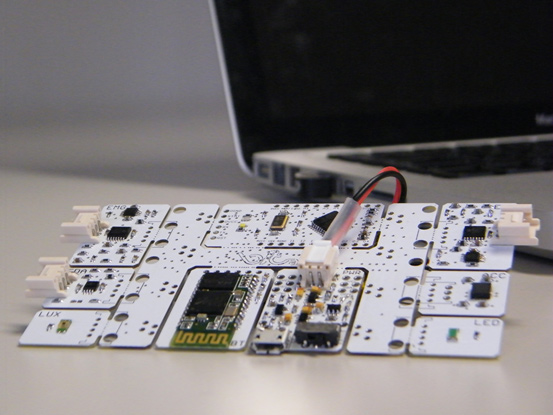
\includegraphics[width=\textwidth]{imagenes//bitalino.jpg}
	\caption{Tarjeta BITalino}
\end{figure}

\section{Aplicaciones de uso comercial}
\subsection{Gazepoint}

\section{Aplicaciones open source para el sensado de señales bioelectricas}


\section{Diseño centrado en el usuario}

En la ingeniería de desarrollo de software la parte fundamental a evaluar es que el sistema funcione (“que haga lo que se espera que haga”). En la mayoría de los casos el usuario final no tiene interacción con el sistema hasta el momento en que el producto es entregado, por lo tanto las características y funcionalidades requeridas por el usuario no son del todo satisfechas. 

	
	La principal diferencia del DCU frente a otros enfoques es que su proceso no es secuencial o lineal, sino que su proceso es iterativo, se realizan ciclos en las prueba del diseño y se optimizan hasta alcanzar el nivel de calidad requerido por el usuario \cite{montero}.

\subsection{Experiencia de usuario}

La experiencia de usuario, también conocida como UX (user experience) se centra en la experiencia del usuario final, incluidas sus percepciones, emociones al interactuar con el producto o sistema. Incluye criterios como la facilidad de uso, la accesibilidad y la satisfacción.

\subsection{Usabilidad}

La usabilidad se refiere a la facilidad con que las personas o los usuarios pueden utilizar una herramienta en particular.  El término usabilidad es un anglicismo que significa facilidad de uso (Bevan, 1995). La ISO/IEC 9126 (ISO/IEC, 2001) define usabilidad como la capacidad de un software de ser comprendido, aprendido, usado y ser atractivo para el usuario, en condiciones específicas de uso. 

	Dentro de la IHC el término usabilidad se refiere a la facilidad con que los usuarios pueden interactuar con el sistema, por ejemplo, para comprobar qué efecto puede tener el uso de la interfaz en el usuario, e identificar qué emociones y estados cognitivos positivos  experimentan los usuarios al realizar tareas específicas.

\section{Frameworks Ux}
\subsection{Framework}

Un framework o marco de trabajo es una base para la elaboración de proyectos. Es un conjunto de herramientas, técnicas y criterios estandarizados  que sirve como guía o plantilla en el desarrollo de software. 


\subsection{Design Thinking}

Design Thinking o Pensamiento de diseño es una metodología centrada en las personas que emplea la susceptibilidad y los métodos del diseñador para crear soluciones innovadoras y tecnológicamente factibles en base a las necesidades del cliente \cite{tim}.


\subsection{ Fases de Design Thinking}
Design Thinking es  un proceso iterativo que sirve para definir y resolver problemas complejos, este proceso se compone de cinco fases: empatizar, definir, idear, prototipar y testear.
\begin{figure}[htb]
	\centering
	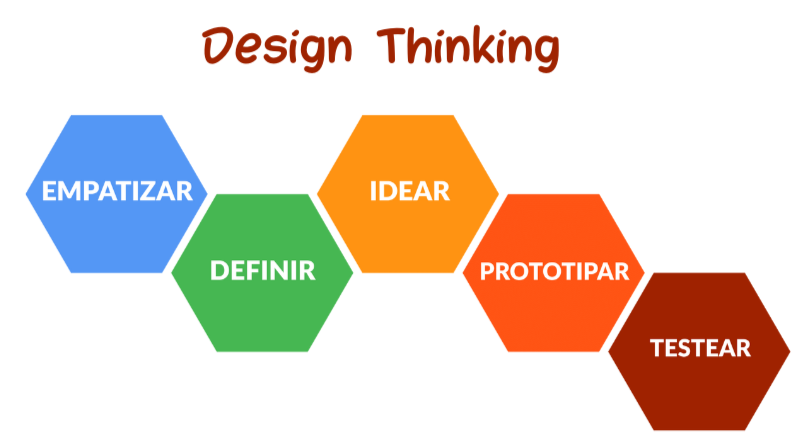
\includegraphics[width=\textwidth]{imagenes//Design_Thinking.png}
	\caption{Etapas de Design Thinking}
\end{figure}

\subsubsection{Empatizar} 

La primera etapa de Design Thinking busca comprender al cliente, entender sus requerimientos y necesidades. El diseñador debe ser capaz de ponerse en el lugar del cliente para entender el problema y generar soluciones acorde a sus necesidades. 

\subsubsection{Definir} 

En esta etapa se debe definir el problema en base a la información recopilada en la etapa de empatía. El diseñador debe ser capaz de extraer lo que realmente genere valor para definir claramente el problema.  

\subsubsection{Idear} 
 
El objetivo de esta fase es crear soluciones potenciales para la resolución del problema especificado. Durante la fase de ideación se genera una lluvia de ideas para obtener un sinfín de posibles soluciones. 

\subsubsection{Prototipar} 
 
En la etapa de prototipado se hacen realidad las ideas generadas en la fase anterior. En esta etapa se construyen prototipos económicos de la posible solución. Los prototipos hacen que se puedan visualizar las ideas, y generar cambios necesarios antes de llegar al resultado final. 

\subsubsection{Testear} 
 
Durante esta fase, se probarán los prototipos con los usuarios implicados. La etapa de prototipado y prueba son las fases más iterativas. Los prototipos se probarán  y reconstruirán hasta alcanzar la solución deseada por el cliente. 

\subsection{Double Diamond}

Método de pensamiento de diseño lanzado en 2004, por Design Council (Consejo de Diseño). Double Diamond es una metodología de innovación que ofrece una descripción clara y completa del proceso de diseño. El Double Diamond es representado por dos diamantes implica un proceso de exploración e investigación profunda (pensamiento divergente) y la toma de acción (proceso convergente).

\begin{figure}[htb]
	\centering
	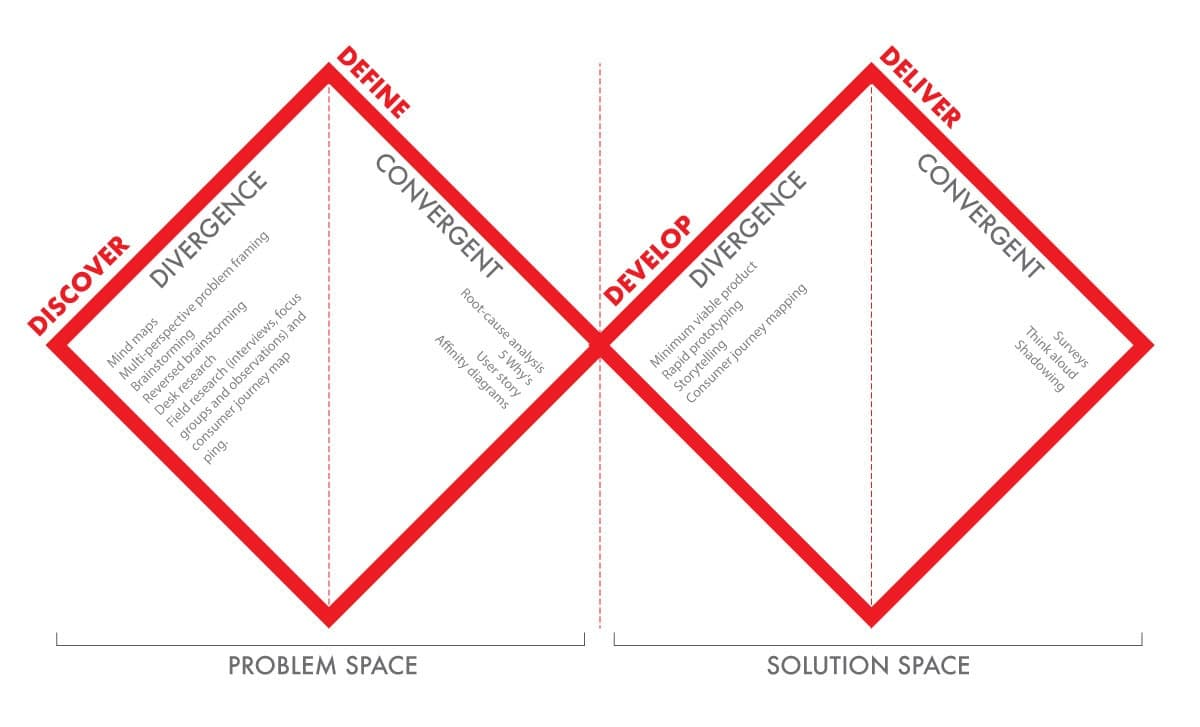
\includegraphics[width=\textwidth]{imagenes//Double_Diamond.jpg}
	\caption{Double Diamond Ux}
\end{figure}

El primer diamante se le conoce como espacio del problema. Es este primer diamante es donde se explora, sintetiza y define el problema. El segundo diamante denominado espacio de soluciones es donde se prueban, iteran, ejecutan las soluciones. El proceso de diseño del Double Diamond se divide en cuatro fases: 

\subsubsection{Descubrir}
Se realiza en el primer diamante, etapa de exploración e investigación. Implica relacionarse con los usuarios para comprender el problema.

\subsubsection{Definir}
En base a la información recopilada en la fase de descubrimiento se define el problema.

\subsubsection{Desarrollar}
Esta fase se  implementa en el segundo diamante, se generan soluciones al problema previamente definido.

\subsubsection{Entregar}
Implica probar las diferentes soluciones a pequeña escala, realizar los cambios y mejoras.

\subsection{Lean UX}

Lean Ux es un enfoque de diseño introducido por  Jeff Gothelf. Lean Ux combina los principios fundamentales de Design Thinking, Lean Startup, Desarrollo de software Agil. 
Lean Ux es una metodología de Pensamiento de Diseño pero no necesariamente se centra en el resultado, sino en el proceso.  En lean Ux se enfoca en un trabajo colaborativo que contempla suposiciones e hipótesis que deben ser validadas. Lean Ux plantea un ciclo de diseño que se divide en tres etapas:

\begin{figure}[htb]
	\centering
	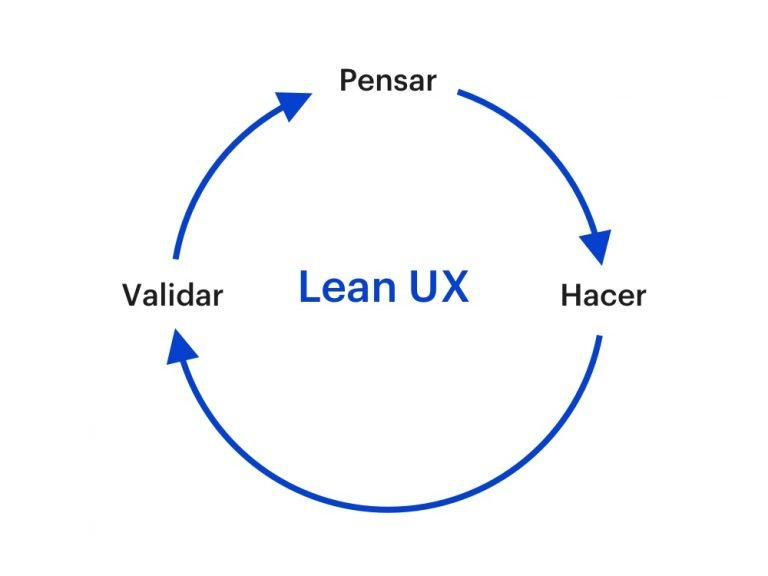
\includegraphics[width=\textwidth]{imagenes//LeanUx.jpg}
	\caption{Proceso Lean Ux}
\end{figure}

\subsubsection{Pensar} 
Esta etapa se enfoca en comprender el problema y generar una hipótesis sobre las posibles soluciones. Este se incluyen sesiones de búsquedas, planteamiento de hipótesis y la creación de usuarios y de modelos mentales.
\subsubsection{Hacer}
En la etapa de hacer, el equipo se dedica a la construcción se soluciones en base a las hipótesis planteadas en la etapa anterior. Esta etapa contempla la generación de prototipos y definición de la propuesta de valor. 
\subsubsection{Validar}
En esta última fase se busca poner a prueba las soluciones propuestas. Probar los prototipos con los usuarios finales para obtener datos concretos y fiables de la funcionalidad del producto.


\section{Modelos de proceso evolutivo}
\subsection{Prototipado}
El modelo de prototipos o modelo de desarrollo evolutivo es usado en el desarrollo de proyectos de software. Consiste en la construcción de prototipos que ayuda a darle al cliente una vista preliminar del software. Este modelo es básicamente prueba y error, ya que si el usuario no está conforme con el resultado significa fallo por lo cual se debe corregir hasta que el usuario quede satisfecho. 
A continuación se mencionan las etapas del modelo de prototipado: 
\begin{itemize}

\item Comunicación con el cliente.
\item Modelado (diseño) del prototipo.
\item Construcción del prototipo.
\item Desarrollo del prototipo.
\item Entrega y retroalimentación del cliente.
\item Entrega del desarrollo final.
\end{itemize}




\subsubsection{Scrum}
Es una metodología que permite el trabajo colaborativo en equipos. Es una metodología ágil que permite a los equipos desarrollar proyectos en pequeños incrementos. Scrum se caracteriza por dividir los proyectos en partes llamadas “sprints” . 

Scrum es un marco de trabajo en equipo.Scrum es una metodología ágil, que consta de reuniones, roles y herramientas que permiten a los equipos trabajar de forma colaborativa. 


\section{Tecnologias de desarrollo}
